\documentclass[aspectratio=169,10pt]{beamer}
\usepackage[T1]{fontenc}
\usepackage{lmodern,amsmath,booktabs,graphicx}
\usetheme{default}
\usecolortheme{dove}
\setbeamercolor{structure}{fg=green!35!black}
\setbeamercolor{frametitle}{fg=green!30!black}
\setbeamertemplate{navigation symbols}{}
\setbeamertemplate{footline}[frame number]
% Generated from audited results; do not edit numeric values manually.
\newcommand{\DefaultReturn}{\ensuremath{-1.417 \pm 0.044}}
\newcommand{\DefaultCVR}{\ensuremath{0.068 \pm 0.025}}
\newcommand{\DefaultEnergy}{\ensuremath{13.989 \pm 0.432}}
\newcommand{\ThermostatEnergy}{14.939}
\newcommand{\ThermostatCVR}{0.010}
\newcommand{\AbstractFinding}{The highest observed mean PPO return is -1.377 for lambda=0.99; rankings are descriptive given only three training seeds.}
\newcommand{\LearningFinding}{Across the default runs, mean validation return changes from -839.501 before training to -1.551 at the final budget. The strongest mean validation point is -1.365; its difference from the final point is retained by the evaluation protocol. Thus a longer budget does not justify assuming that every run's final policy is its best policy.}
\newcommand{\PerformanceFinding}{The default uses 6.4 percent less electricity than the thermostat reference. Its CVR is 0.058 percentage points higher. Among PPO configurations, lambda=0.99 has the highest observed mean return (-1.377), with 0.056 percent CVR and 13.608 kWh. This is an observed grid ranking, not a test-based choice used to retrain or select checkpoints.}
\newcommand{\ClipFinding}{Mean final-test returns for clip ranges 0.1, 0.2, and 0.3 are -1.508, -1.417, -1.929, respectively. Corresponding mean update KL estimates are 0.002838, 0.008136, 0.0245. The largest clip's weakest seed is 2, at -2.866; this run is retained in all summaries. Relative to the same seed labels at the default, clip=0.1 improves return in 0 of 3 pairs (mean difference -0.091). These diagnostics describe realized updates and do not establish a hard trust-region constraint.}
\newcommand{\LambdaFinding}{At lambda 0.90, 0.95, and 0.99, mean final-test returns are -1.501, -1.417, -1.377. Across-seed return standard deviations are 0.162, 0.044, 0.030. Relative to the same seed labels at the default, lambda=0.99 improves return in 3 of 3 pairs (mean difference +0.040). This changes the advantage estimator at fixed gamma; its ranking should not be extrapolated to every thermal timescale or value-function accuracy.}
\newcommand{\EpochFinding}{Five, ten, and twenty epochs give final-test returns of -1.447, -1.417, -1.441. The corresponding optimization counts are 40,000, 80,000, and 160,000 mini-batch steps. Default has the highest observed mean return within this slice; additional optimization is not intrinsically a guarantee of better closed-loop control.}
\newcommand{\StabilityFinding}{The default's mean late-validation standard deviation is 0.160. The largest mean late peak-to-final drop occurs for Default (0.195 return units).}
\newcommand{\RuntimeFinding}{Mean training wall times excluding periodic validation are 113.3 seconds, 129.4 seconds, 194.5 seconds for 5, 10, and 20 epochs, respectively.}
\newcommand{\ConclusionFinding}{Within the frozen seven-configuration experiment, lambda=0.99 achieves the highest observed mean final-test return. The default's physical outcomes are 0.068 percent CVR, 0.018 degree-hours, and 13.989 kWh per seven-day episode. Relative to the thermostat, it uses 6.4 percent less electricity; the comfort comparison must be considered separately. The principal result is a task-specific account of sample efficiency, comfort--energy balance, update variability, and computational cost, rather than a universal optimal PPO setting.}
\newcommand{\CoverageFinding}{The finite tables have unequal weather-offset coverage (validation versus test, degrees C): hot: [-1.75, -0.94] versus [-1.78, 1.11]; transition: [-1.82, -0.44] versus [-1.57, 1.91]. These conditions remain within training support, but validation rankings need not match test rankings. In particular, the largest-clip run with seed 2 has appreciably worse final-test control in some hot and transition conditions. An independent model reload reproduces its test metrics exactly; it is retained without retuning the protocol.}
\newcommand{\TrajectoryFinding}{For these fixed cold, hot, and transition examples, the default PPO's median indoor temperatures are 21.02, 24.88, 21.84 degrees C, respectively. The comfort bands and thermostat setpoints supply context for where the learned controller operates. Cumulative electricity is monotone and ends at the episode energy; temperature boundary crossings and action changes should be interpreted jointly rather than equated with instability on their own.}
\newcommand{\SlidePerformance}{Default: 0.07 percent CVR, 13.99 kWh; thermostat: 0.01 percent, 14.94 kWh.}
\newcommand{\SlideClip}{Mean return, small/default/large: -1.508, -1.417, -1.929.}
\newcommand{\SlideLambda}{Mean return, small/default/large: -1.501, -1.417, -1.377.}
\newcommand{\SlideEpochs}{Mean training time, 5/10/20 epochs: 113/129/195 seconds.}
\newcommand{\SlideStability}{Largest mean late-validation peak-to-final drop: Default, 0.19 return units.}
\newcommand{\SlideConclusion}{Highest observed mean PPO return: lambda=0.99 (-1.377); this is a descriptive grid result.}

% Replace this line when the three team members provide names and student IDs.
\newcommand{\TeamAuthors}{Team member names and student IDs to be supplied}

\title{PPO Hyperparameters for Room HVAC Control}
\subtitle{Clip range, GAE lambda, and update epochs}
\author{\TeamAuthors}
\institute{AIAA 5034 --- Topic 16}
\date{Fall 2026}
\begin{document}
\begin{frame}
\titlepage
\end{frame}

\begin{frame}{A small physical model with delayed effects}
\begin{columns}
\column{.55\textwidth}
\begin{align*}
C_i\dot T_i&=(T_e-T_i)/R_{ie}+Q_{\rm hvac}+Q_g\\
C_e\dot T_e&=(T_o-T_e)/R_{eo}+(T_i-T_e)/R_{ie}
\end{align*}
\begin{itemize}
\item Two equivalent temperatures; stored heat causes inertia.
\item 11 observations, one continuous heating/cooling action.
\item 15-minute control; seven-day episodes.
\end{itemize}
\column{.42\textwidth}
\begin{block}{Fixed objective}
$r_t=-\Delta t\,d_t-0.1E_t$
\end{block}
\begin{itemize}
\item Comfort violations: CVR and degree-hours.
\item Electricity: kWh.
\item Model and physical tests supplied by teammate.
\end{itemize}
\end{columns}
\end{frame}

\begin{frame}{PPO: three parameters, three stages}
\begin{enumerate}
\item Collect a rollout using the current actor and value network.
\item Estimate advantages using GAE: \textbf{lambda}.
\item Optimize the clipped policy objective: \textbf{clip range}.
\item Repeat mini-batch optimization: \textbf{epochs}.
\end{enumerate}
\vspace{2mm}
\[
\hat A_t=\sum_l(\gamma\lambda)^l\delta_{t+l},\qquad
L^{\rm clip}=\mathbb E\big[\min(\rho\hat A,\mathrm{clip}(\rho,1-\epsilon,1+\epsilon)\hat A)\big]
\]
\begin{itemize}
\item Separate two-layer 64-unit actor/critic MLPs; 9,987 parameters.
\item Observe raw physical metrics; freeze normalization at evaluation.
\item Clipping is a surrogate objective, not a hard KL bound.
\end{itemize}
\end{frame}

\begin{frame}{A controlled and reproducible comparison}
\begin{columns}
\column{.49\textwidth}
\begin{tabular}{lccc}
\toprule Factor & Small & Default & Large\\\midrule
Clip range & 0.1 & 0.2 & 0.3\\
GAE lambda & 0.90 & 0.95 & 0.99\\
Epochs & 5 & 10 & 20\\\bottomrule
\end{tabular}
\vspace{3mm}
\begin{itemize}
\item One factor at a time: 7 configurations.
\item 3 seeds each: 21 seeded runs.
\item 512,000 interactions per run.
\end{itemize}
\column{.47\textwidth}
\begin{itemize}
\item Separate fixed validation and test conditions.
\item 30 final conditions, balanced across weather.
\item Final checkpoint, without test-based selection.
\item Same conditions for off and thermostat rules.
\item M4 CPU, 16 GB; two processes under screen.
\end{itemize}
\end{columns}
\end{frame}

\begin{frame}{Learning: avoid discomfort first, then refine control}
\centering
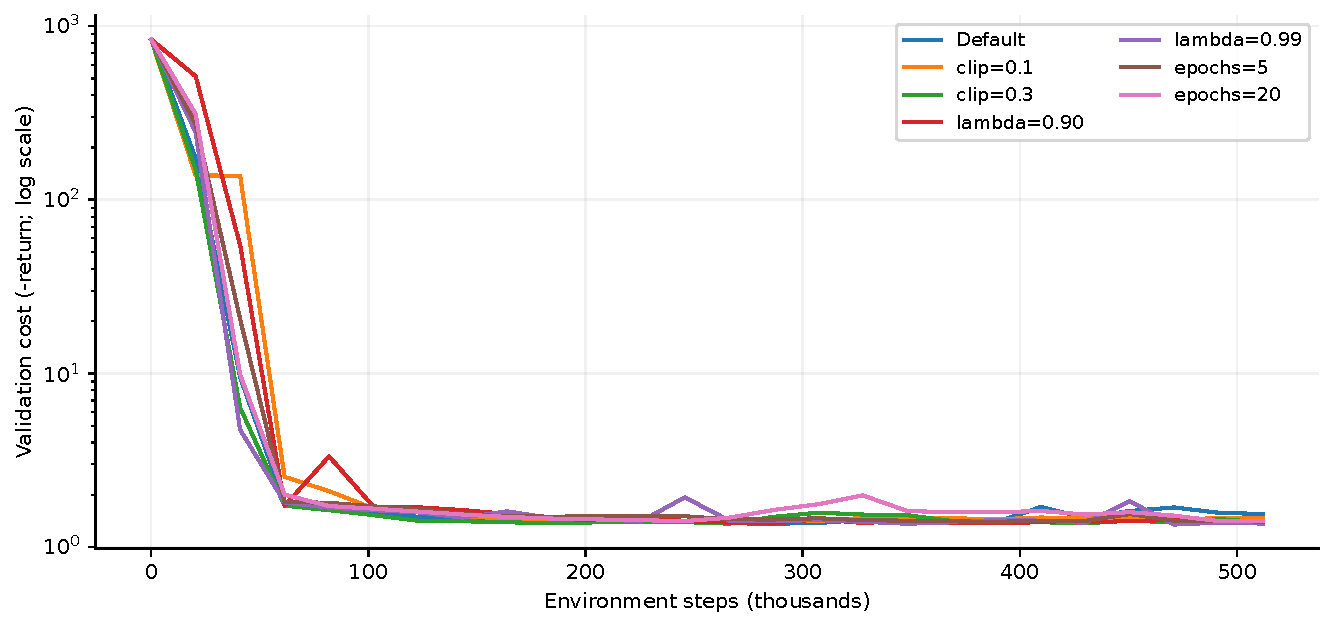
\includegraphics[width=.85\linewidth,height=.64\textheight,keepaspectratio]{../../results/figures/slides_learning.pdf}
\par\small Across-seed means; logarithmic cost axis. Full return curves and seed variability are in the report.
\end{frame}

\begin{frame}{Final test: comfort and electricity must be reported separately}
\centering
{\scriptsize
\begin{tabular}{lrrr}
\toprule Controller & Return & CVR (\%) & kWh \\
\midrule
HVAC off & -873.78 & 80.72 & 0.00 \\
Thermostat & -1.50 & 0.01 & 14.94 \\
\midrule
Default & \ensuremath{-1.42 \pm 0.04} & \ensuremath{0.07 \pm 0.02} & \ensuremath{13.99 \pm 0.43} \\
clip=0.1 & \ensuremath{-1.51 \pm 0.05} & \ensuremath{1.55 \pm 0.24} & \ensuremath{13.76 \pm 0.14} \\
clip=0.3 & \ensuremath{-1.93 \pm 0.81} & \ensuremath{3.29 \pm 4.85} & \ensuremath{13.76 \pm 0.52} \\
lambda=0.90 & \ensuremath{-1.50 \pm 0.16} & \ensuremath{0.73 \pm 1.17} & \ensuremath{13.95 \pm 0.56} \\
lambda=0.99 & \ensuremath{-1.38 \pm 0.03} & \ensuremath{0.06 \pm 0.00} & \ensuremath{13.61 \pm 0.28} \\
epochs=5 & \ensuremath{-1.45 \pm 0.05} & \ensuremath{0.19 \pm 0.23} & \ensuremath{14.26 \pm 0.52} \\
epochs=20 & \ensuremath{-1.44 \pm 0.05} & \ensuremath{0.05 \pm 0.01} & \ensuremath{14.26 \pm 0.46} \\
\bottomrule
\end{tabular}
}

\vspace{2mm}
\begin{itemize}
\item PPO: means $\pm$ sample SD across training seeds, after averaging conditions.
\item A higher weighted return need not improve both physical metrics.
\item \SlidePerformance{}
\end{itemize}
\end{frame}

\begin{frame}{Clip range: changing the policy-update objective}
\centering
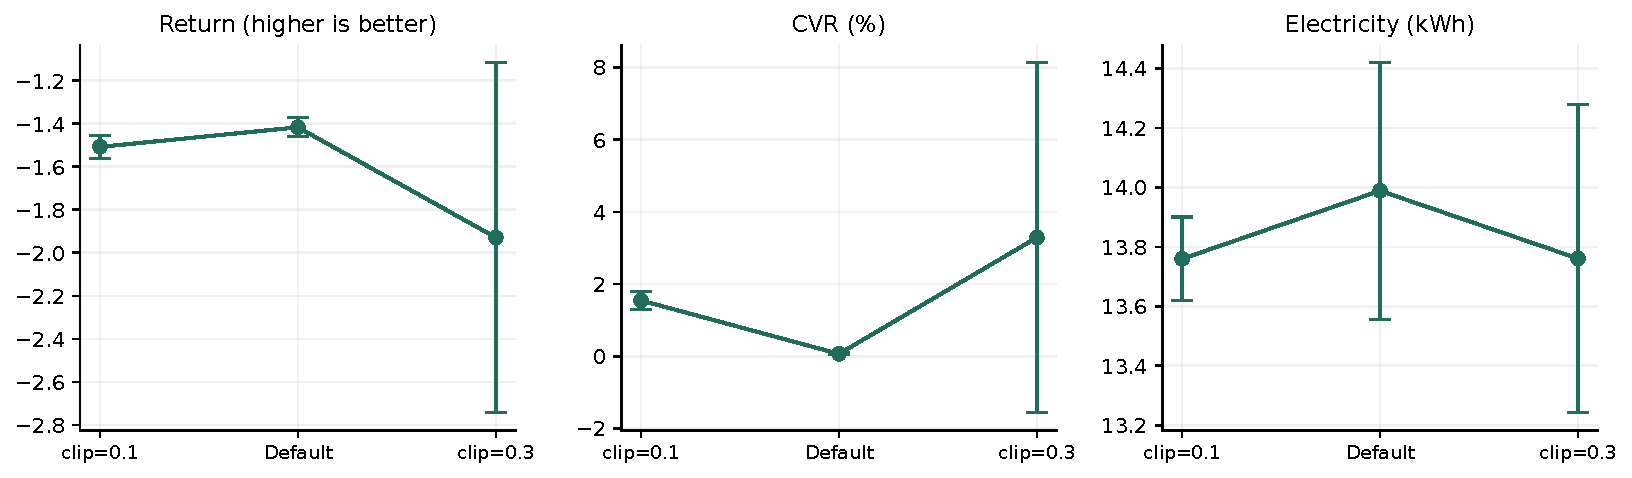
\includegraphics[width=\linewidth]{../../results/figures/slides_clip.pdf}
\begin{itemize}
\item Smaller clipping discourages large favorable probability-ratio changes earlier.
\item \SlideClip{}
\end{itemize}
\end{frame}

\begin{frame}{GAE lambda: changing the advantage estimate}
\centering
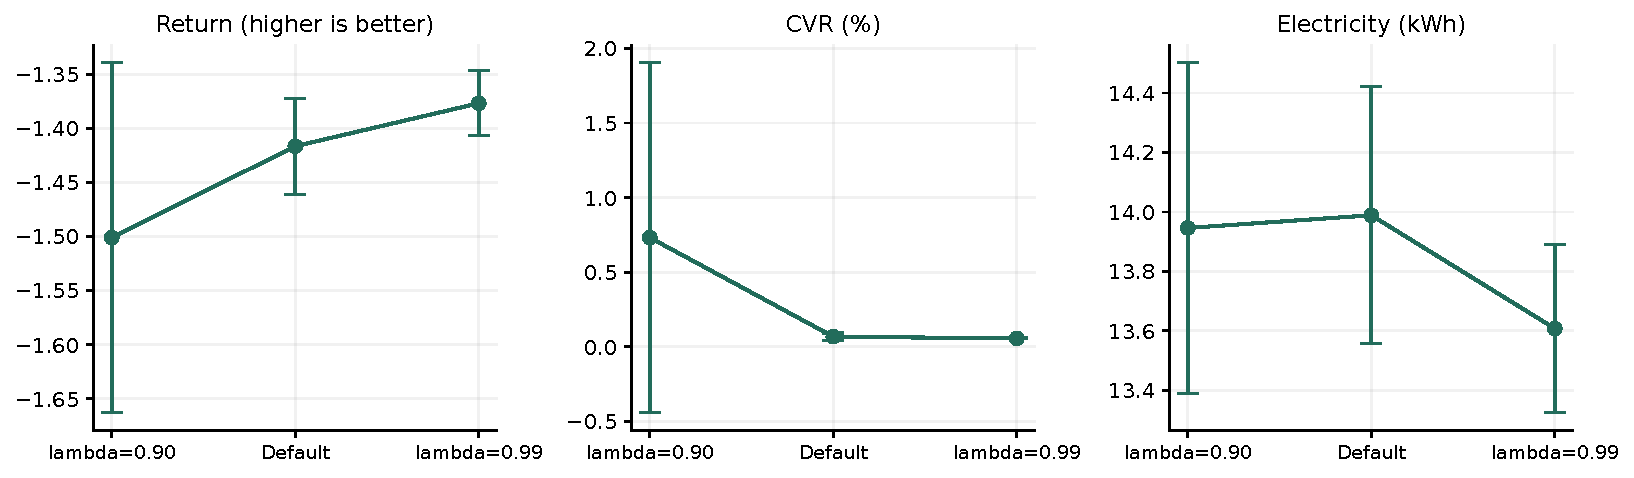
\includegraphics[width=\linewidth]{../../results/figures/slides_lambda.pdf}
\begin{itemize}
\item Larger lambda uses longer reward fragments; value errors and variance matter.
\item \SlideLambda{}
\end{itemize}
\end{frame}

\begin{frame}{Epochs: data reuse also changes computation}
\centering
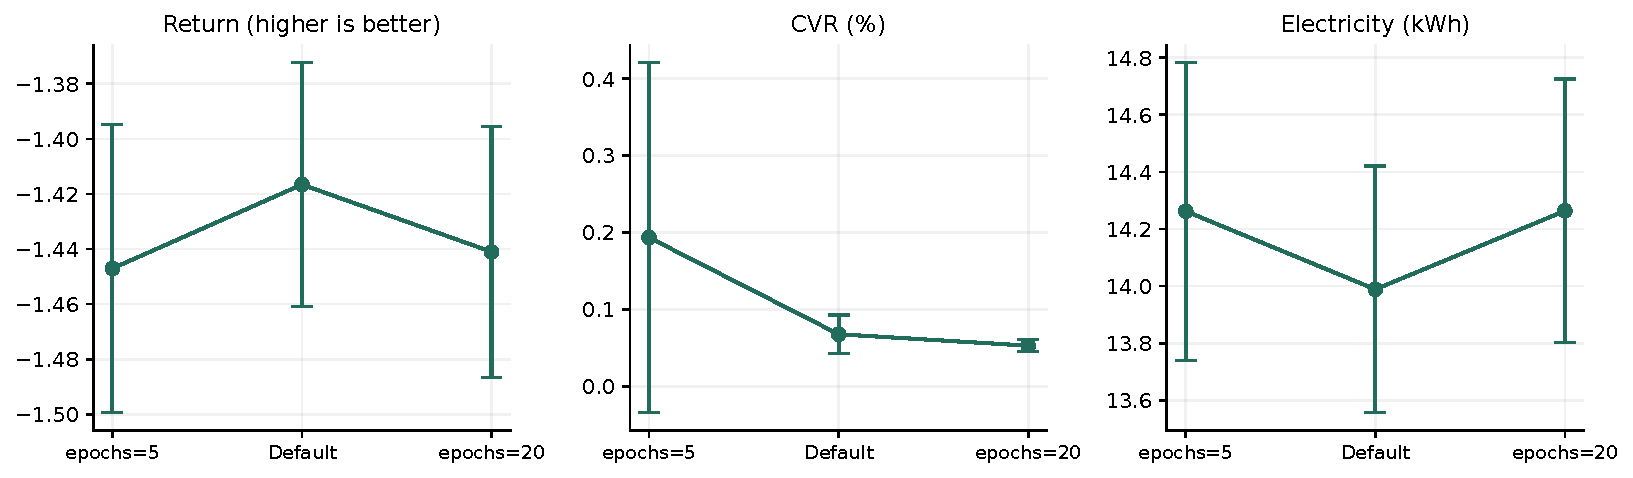
\includegraphics[width=\linewidth]{../../results/figures/slides_epochs.pdf}
\begin{itemize}
\item 5/10/20 epochs: 40k/80k/160k optimizer steps at the same sample budget.
\item \SlideEpochs{}
\end{itemize}
\end{frame}

\begin{frame}{A preselected cold-weather trajectory}
\centering
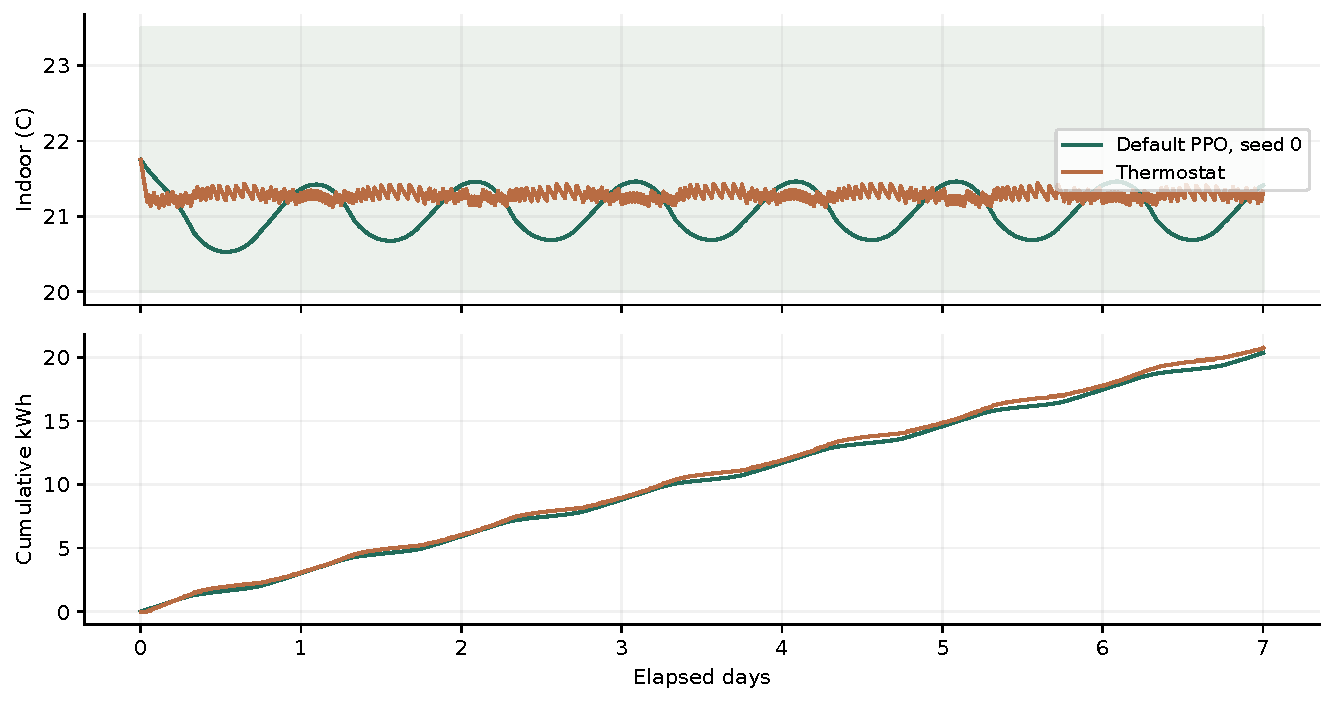
\includegraphics[width=.82\linewidth,height=.73\textheight,keepaspectratio]{../../results/figures/slides_cold_trace.pdf}
\par\small Condition \texttt{test\_cold\_00}; default PPO seed 0. Other scenes and executed actions are in the report.
\end{frame}

\begin{frame}{Stability and limits of the evidence}
\begin{itemize}
\item Fixed final checkpoints retain late deterioration instead of hiding it.
\item \SlideStability{}
\item KL, clipped fraction, late fluctuations and seed spread are complementary diagnostics.
\item Sparse validation misses some warmer offsets; final tests expose this sensitivity.
\item Only three training seeds; descriptive rankings, not significance claims.
\item Synthetic weather, constant COP, fully observed thermal state.
\item Single-factor design does not resolve all hyperparameter interactions.
\end{itemize}
\end{frame}

\begin{frame}{Conclusions and questions}
\begin{itemize}
\item \SlideConclusion{}
\item Comfort, energy, learning progress and compute cost need separate assessment.
\item Complete local workflow: tested model, shared evaluation, audited runs and reproducible plots.
\item Next steps: more seeds, limited interaction study, and realistic thermal/equipment data.
\end{itemize}
\vspace{5mm}
\centering\Large Questions?
\end{frame}
\end{document}
